\documentclass{ltjsarticle}
\RequirePackage{luatex85}
\usepackage[utf8]{inputenc}
\usepackage[dvipdfmx]{color}
\usepackage{enumerate}
\usepackage{here}
\usepackage{amsthm}
\usepackage{amsfonts}
\usepackage{amsmath}
\usepackage{amssymb}
\usepackage{latexsym}
\usepackage{ytableau}
\usepackage{docmute}
\usepackage{mathtools}
\usepackage{xr}
\usepackage{tikz}
\usetikzlibrary{intersections, calc, arrows.meta}
\usepackage[all]{xy}
\usepackage{graphics}
\usepackage[luatex]{hyperref}
%\usepackage{pxjahyper}



\theoremstyle{definition}
\newtheorem{defin}{定義}[subsection]
\newtheorem{theo}[defin]{定理}
\newtheorem{cor}[defin]{系}
\newtheorem{prop}[defin]{命題}
\newtheorem{lemm}[defin]{補題}
\newtheorem{notice}[defin]{注意}
\newtheorem{eg}[defin]{例}
\newtheorem{fact}[defin]{事実}


\renewcommand{\labelenumi}{(\roman{enumi})}


\newcommand{\invlimit}{\mathop{\lim_{\longleftarrow}}}
\newcommand{\dirlimit}{\mathop{\lim_{\longrightarrow}}}
\newcommand{\ind}{\text{Ind}}
\newcommand{\Hom}{\text{Hom}}
\newcommand{\tr}{\text{tr}}
\newcommand{\id}[1]{\text{id}_{#1}}
\newcommand{\sgn}{\mathrm{sgn}}
\newcommand{\res}[1]{\text{Res}_{#1}}
\newcommand{\generated}[1]{\langle\:#1\:\rangle}
\newcommand{\im}{\text{Im }}
\newcommand{\rank}{\text{rank }}
\newcommand{\del}[2]{\frac{\partial #1}{\partial #2}}
\newcommand{\delsametwo}[2]{\frac{\partial^2 #1}{\partial #2^2}}
\newcommand{\delothertwo}[3]{\frac{\partial^2#1}{\partial#2\partial#3}}
\newcommand{\ddel}[2]{\frac{\partial}{\partial #2}#1}
\newcommand{\ddelsametwo}[3]{\frac{\partial^2}{\partial #2^2}#1}
\newcommand{\ddelothertwo}[3]{\frac{\partial^2}{\partial#2\partial#3}#1}
\newcommand{\simneq}{\not\simeq}
\newcommand{\transpose}[1]{^t\!#1}
\newcommand{\ie}{\text{i.e.}}
\newcommand{\inv}[1]{#1^{-1}}
\newcommand{\real}{\mathbb{R}}
\newcommand{\complex}{\mathbb{C}}
\newcommand{\integer}{\mathbb{Z}}
\newcommand{\quotient}{\mathbb{Q}}
\newcommand{\natnum}{\mathbb{N}}
\newcommand{\proj}{\mathbb{P}}
\newcommand{\affine}{\mathbb{A}}
\newcommand{\tensor}[3]{#1\otimes_#2#3}
\newcommand{\map}[3]{#1:#2\rightarrow#3}
\newcommand{\aut}[2]{\mathrm{Aut}_{#1} (#2)}
\newcommand{\hommoph}[2]{\mathrm{Hom}_{#1}(#2)}
\newcommand{\gl}{\text{GL}}
\newcommand{\End}{\text{End}}
\newcommand{\set}[2]{\left\{\:#1\:\middle|\:#2\:\right\}}
\newcommand{\pmat}[1]{\begin{pmatrix} #1
\end{pmatrix}}
\newcommand{\vmat}[1]{\begin{vmatrix} #1
\end{vmatrix}}
\newcommand{\bmat}[1]{\begin{bmatrix} #1
\end{bmatrix}}
\newcommand{\br}{\vskip\baselineskip}
\newcommand{\Lie}{\text{Lie}}
\newcommand{\Sym}{\text{Sym}}
\newcommand{\Alt}{\text{Alt}}
\newcommand{\ch}{\text{ch}}
\newcommand{\diag}{\text{diag}}
\newcommand{\comb}[2]{_{#1}C_{#2}}
\newcommand{\codim}{\text{codim}\:}
\newcommand{\yd}[1]{\ydiagram{#1}}

\title{aaa}
\author{}
\date{}


\begin{document}
\maketitle

\begin{figure}[ht]
  \centering
  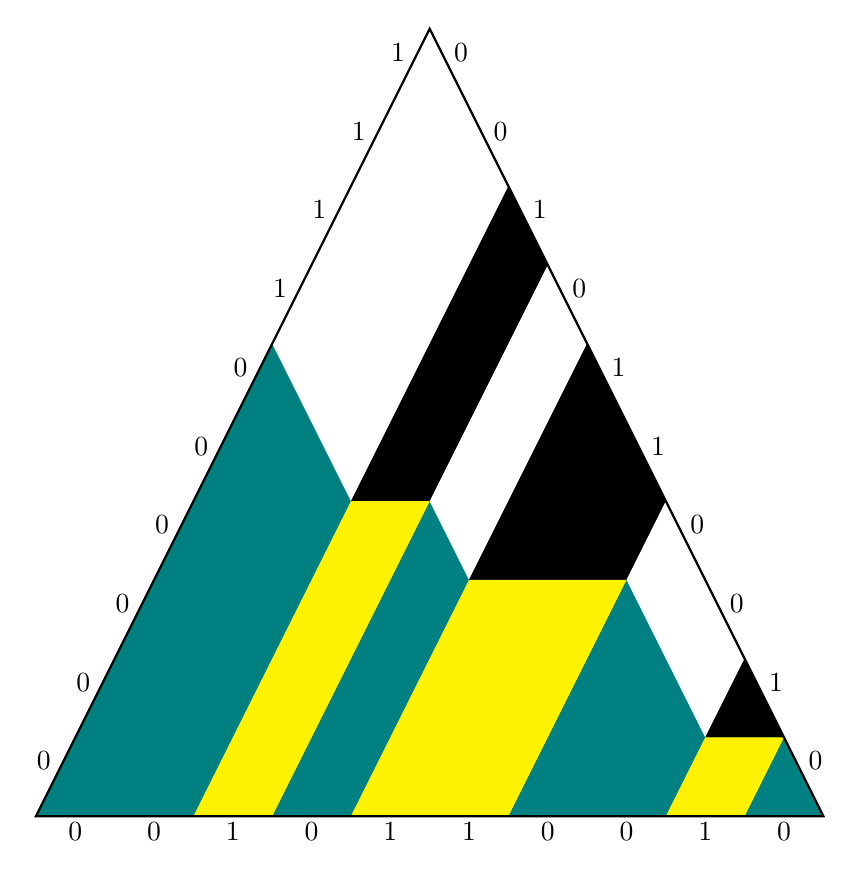
\begin{tikzpicture}
    \fill[teal] (0,0)--(10,0)--(5,10)--cycle;
    \fill[white] (5,10)-- ++(1,-2)-- ++(-2,-4)-- ++(-1,2)--cycle;
    \fill[black] (6,8)-- ++(1/2,-1)-- ++(-3/2,-3)-- ++(-1,0)--cycle;
    \fill[white] (6.5,7)-- ++(1/2,-1)-- ++(-3/2,-3)-- ++(-1/2,1)--cycle;
    \fill[black] (7,6)-- ++(1,-2)-- ++(-1/2,-1)-- ++(-2,0)--cycle;
    \fill[white] (8,4)-- ++(1,-2)-- ++(-1/2,-1)-- ++(-1,2)--cycle;
    \fill[black] (9,2)-- ++(1/2,-1)-- ++(-1,0)--cycle;

    \fill[yellow] (5,4)-- ++(-2,-4)-- ++(-1,0)-- ++(2,4)--cycle;
    \fill[yellow] (7.5,3)-- ++(-3/2,-3)-- ++(-2,0)-- ++(3/2,3)--cycle;
    \fill[yellow] (9.5,1)-- ++(-1/2,-1)-- ++(-1,0)-- ++(1/2,1)--cycle;

    \node at (0.1,0.7) {$0$};
    \node at (0.1 + 1/2, 0.7+1) {$0$};
    \node at (0.1 + 2/2, 0.7+2) {$0$};
    \node at (0.1 + 3/2, 0.7+3) {$0$};
    \node at (0.1 + 4/2, 0.7+4) {$0$};
    \node at (0.1 + 5/2, 0.7 + 5) {$0$};
    \node at (0.1 + 3, 0.7 + 6) {$1$};
    \node at (0.1 + 3 + 1/2, 0.7 + 7) {$1$};
    \node at (0.1 + 3 + 2/2, 0.7 + 8) {$1$};
    \node at (0.1 + 4 + 1/2, 0.7 + 9) {$1$};

    \node at (5.4, 9.7) {$0$};
    \node at (5.4 + 1/2, 9.7 - 1) {$0$};
    \node at (5.4 + 2/2, 9.7 - 2) {$1$};
    \node at (5.4 + 3/2, 9.7 - 3) {$0$};
    \node at (5.4 + 4/2, 9.7 - 4) {$1$};
    \node at (5.4 + 5/2, 9.7 - 5) {$1$};
    \node at (5.4 + 6/2, 9.7 - 6) {$0$};
    \node at (5.4 + 7/2, 9.7 - 7) {$0$};
    \node at (5.4 + 8/2, 9.7 - 8) {$1$};
    \node at (5.4 + 9/2, 9.7 - 9) {$0$};

    \node at (1/2,-0.2) {$0$};
    \node at (1/2 + 1,-0.2) {$0$};
    \node at (1/2 + 2,-0.2) {$1$};
    \node at (1/2 + 3,-0.2) {$0$};
    \node at (1/2 + 4,-0.2) {$1$};
    \node at (1/2 + 5,-0.2) {$1$};
    \node at (1/2 + 6,-0.2) {$0$};
    \node at (1/2 + 7,-0.2) {$0$};
    \node at (1/2 + 8,-0.2) {$1$};
    \node at (1/2 + 9,-0.2) {$0$};
    

    \draw[thick] (0,0)--(10,0)--(5,10)--cycle;
  \end{tikzpicture}
  \caption{$\mu=0010110010$の場合の$P_0$} \label{unique puzzle}
\end{figure}

\end{document}